Glitches refer to sporadic large discontinuities in the timing residual as
shown in figure \ref{fig: glitch}.  A glitch is characterised by a sudden and
large increase in the rotation frequency; this is frequently followed by an
exponential `recovery' in which the frequency decays towards the pre-glitch
value. In figure \ref{fig: glitch} we reproduce the essential features of a
glitch and describe them in the caption.  Typically it not possible to produce
a single timing model across a glitch, generally two timing models are used 
either side of a glitch.

\begin{figure}[ htb]
    \centering
    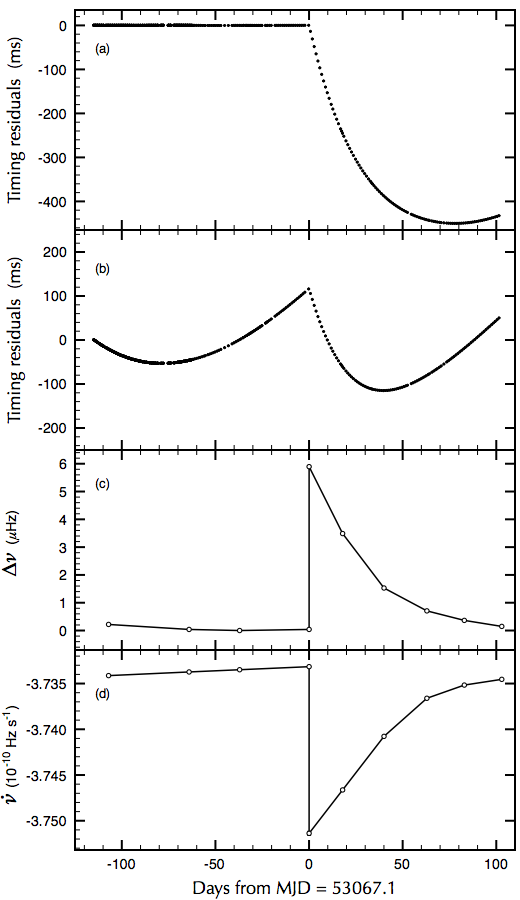
\includegraphics[width=0.6\textwidth]{GlitchExample_jbman}
    \caption{An example of a glitch reproduced from the work of 
            \citet{Espinoza2011}. This shows residuals and fitted coefficients 
            during a glitch for the Crab pulsar (B0531+21). Fitting two Taylor
            expansions either side of the glitch in (a) shows that the pulsar is
            well behaved before the glitch. In (b) the timing residual having 
            fitted a single Taylor expansion over all the data is shown. The 
            frequency residual is given in (c), this illustrates the increase in 
            frequency and the exponential recovery. In the fitted spindown 
            coefficient  plotted in (d) we see a corresponding decrease in spindown
            and exponential recovery.}
    \label{fig: glitch}
\end{figure} 


